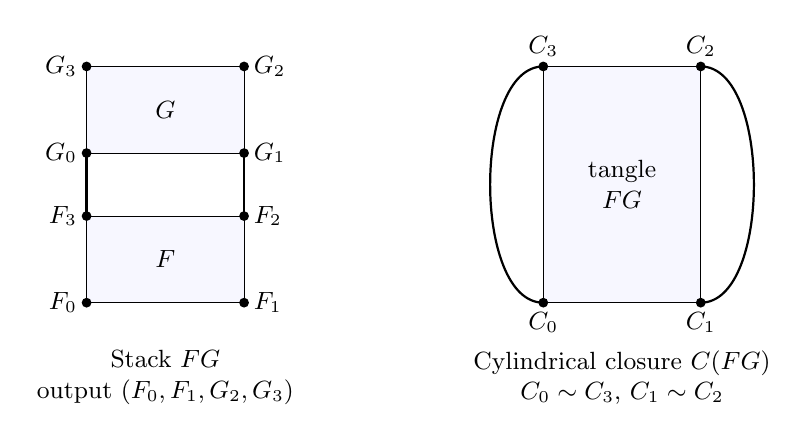
\begin{tikzpicture}[x=1cm,y=1cm, every node/.style={font=\small},
  endpoint/.style={circle,fill,inner sep=1.25pt}]
\begin{scope}
\draw[fill=blue!3] (0,0) rectangle (2,1.1);
\draw[fill=blue!3] (0,1.9) rectangle (2,3);
\node at (1,.55) {$F$}; \node at (1,2.45) {$G$};
\draw[thick] (0,1.1)--(0,1.9) (2,1.1)--(2,1.9);
\foreach \x/\y/\label/\anchor in {0/0/F_0/east,2/0/F_1/west,
  2/1.1/F_2/west,0/1.1/F_3/east,0/1.9/G_0/east,
  2/1.9/G_1/west,2/3/G_2/west,0/3/G_3/east}
  {\node[endpoint] at (\x,\y) {};\node[anchor=\anchor] at (\x,\y) {$\label$};}
\node[align=center] at (1,-.95) {Stack $FG$\\output $(F_0,F_1,G_2,G_3)$};
\end{scope}
\begin{scope}[xshift=5.8cm]
\draw[fill=blue!3] (0,0) rectangle (2,3);
\node[align=center] at (1,1.5) {tangle\\$FG$};
\draw[thick] (0,0)..controls(-.9,0)and(-.9,3)..(0,3);
\draw[thick] (2,0)..controls(2.9,0)and(2.9,3)..(2,3);
\foreach \x/\y/\label/\anchor in {0/0/C_0/north,2/0/C_1/north,
  2/3/C_2/south,0/3/C_3/south}
  {\node[endpoint] at (\x,\y) {};\node[anchor=\anchor] at (\x,\y) {$\label$};}
\node[align=center] at (1,-.95) {Cylindrical closure $C(FG)$\\$C_0\sim C_3$, $C_1\sim C_2$};
\end{scope}
\end{tikzpicture}
